\chapter{Tutorial}

\section{Instalación}

Para la realización de este tutorial, se utilizaron los paquetes \textbf{sp, gstat, geoR}. los cuales se los instala de la siguiente manera:

install.packages(``sp'',``gstat'', ``geoR'', ``geoRglm'', ``RColorBrewer'')

\section{Análisis exploratorio de datos}

El análisis exploratorio de datos comienza con el trazado de mapas con una variable medida, los valores observados los podemos expresar
utilizando el color o tamaño del símbolo.\\

\lstset{backgroundcolor=\color{white},frame=shadowbox, language=R}
\begin{lstlisting}
> library(lattice)
> library(sp)
> data(meuse)
> coordinates(meuse) <- c("x", "y")
> spplot(meuse, "zinc", do.log = T, colorkey = TRUE)
> bubble(meuse, "zinc", do.log = T, key.space = "bottom")
\end{lstlisting}

La estructura evidente aquí es que la concentración de zinc es mayor cerca de la
orilla del río Meuse. En caso de una tendencia espacial evidente, tales como la relación
entre la parte superior de concentración de zinc del suelo y la distancia al río, también 
se puede trazar mapas con valores ajustados y residuales como lo muestra la figura~\ref{fig:figura01}.

\begin{figure}
  \centering
  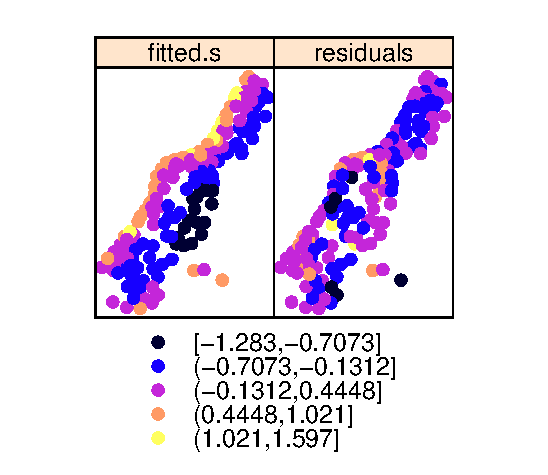
\includegraphics[scale=1]{pictures/figura01.pdf}
  \caption{Mapa trazado con valores ajustados y residuales}
  \label{fig:figura01}
\end{figure}

Los análisis exporatorios se los puede analizar aún más en el contexto de modelos geoestadísticos; aunque primero 
vamos a referirnos a enfoques de interpolación simples y no geoestadísticos.

\section{Métodos de interpolación no geoestadísticos}

Por lo general, la interpolación se realiza en una rejilla regular. Para el conjunto de datos Meuse,
las coordenadas de puntos en una cuadrícula regular ya están definidos en el meuse.grid
data.frame, y se convierten en un SpatialPixelsDataFrame así:
\\
\lstset{backgroundcolor=\color{white},frame=shadowbox, language=R}
\begin{lstlisting}
> data(meuse.grid)
> coordinates(meuse.grid) <- c("x", "y")
> meuse.grid <- as(meuse.grid, "SpatialPixelsDataFrame")
\end{lstlisting}

Alternativamente, podríamos interpolar los puntos individuales, conjuntos de puntos distribuidos irregularmente, 
o para un promedio de más áreas cuadradas o irregulares.

\subsection{Interpolación ponderada de distancia inversa}

Interpolación ponderada basada en la distancia inversa (IDW) calcula un promedio ponderado, 
donde los coeficientes de ponderación para las observaciones son calculados deacuerdo a su distancia a la ubicación de interpolación.

La potencia de la distancia inversa determina el rango en cual punto(s)  más cercano se prefieren sobre
los puntos más distantes; para valores grandes IDW converge a la interpolación de un vecino más cercano.
Puede ajustarse, por ejemplo usando la validación cruzada. IDW también se puede utilizar dentro de los alrededores de búsqueda local.

Debido a que el paquete \textbf{spatstat} también ofrece una función llamada idw, que desambigua los dos, debería \textbf{spatstat} ser cargado
en el espacio de trabajo de la sesión, llamando a la función gstat usando el operador ``::'' para elegir el idw deseado:
\\
\lstset{backgroundcolor=\color{white},frame=shadowbox, language=R}
\begin{lstlisting}
> data(meuse)
> data(meuse.grid)
> coordinates(meuse) <- c("x", "y")
> coordinates(meuse.grid) <- c("x", "y")
> idw.out <- gstat::idw(zinc ~ 1, meuse, meuse.grid, idp = 2.5)
[inverse distance weighted interpolation]
> as.data.frame(idw.out)[1:5, ]
\end{lstlisting}

La variable de salida se llama var1.pred, y los valores de var1.var son NA
porque la distancia inversa no proporciona varianzas de predicción de error.

Resultados de interpolación de distancia inversa generalmente en mapas que son muy similares a los mapas kriged\footnote{Proceso de regresión Gausiana} 
cuando se utiliza un variograma sin o con una pequeña nugget\footnote{La altura del salto de la semivariogram en la discontinuidad en el origen}. En contraste con kriging,
para considerar unicamente distancias a la ubicación de predicciones ignora
la configuración espacial de las observaciones; esto puede dar lugar a efectos no 
deseados si los lugares de observación están fuertemente agrupadas. Otra diferencia es que los pesos están 
garantizados para estar entre 0 y 1, lo que resulta en valores interpolados, nunca fuera del rango de valores observados.

\subsection{Regresión lineal}

Para la predicción espacial utilizando modelos lineales simples, podemos utilizar lm así:
\\
\lstset{backgroundcolor=\color{white},frame=shadowbox, language=R}
\begin{lstlisting}
> zn.lm <- lm(log(zinc) ~ sqrt(dist), meuse)
> meuse.grid$pred <- predict(zn.lm, meuse.grid)
> meuse.grid$se.fit <- predict(zn.lm, meuse.grid, 
+ se.fit = TRUE)$se.fit
\end{lstlisting}

Alternativamente, el método predecir utilizado aquí puede proporcionar los intervalos de predicción o de confianza
para un nivel de confianza dado. Alternativamente, podemos usar la función Krige en gstat para esto.
\\
\lstset{backgroundcolor=\color{white},frame=shadowbox, language=R}
\begin{lstlisting}
> meuse.lm <- krige(log(zinc) ~ sqrt(dist), meuse, meuse.grid)
[ordinary or weighted least squares prediction]
\end{lstlisting}

Esto en este caso no Krige ningún variograma es especificado, pero utiliza lineal
regresión.

Utilizado de esta forma, el resultado es idéntico al de lm. Sin embargo, también se puede utilizar para
predecir con modelos de regresión que estén colocados dentro de los alrededores locales en torno a una ubicación
de predicción o proporcionan valores de las medias pronosticados para las áreas espaciales. La varianza devuelta es la varianza 
de predicción de error en la predicción de puntos o la varianza de estimación de error
cuando se utiliza para bloques.

Se obtiene una forma especial de regresión lineal cuando se utilizan polinomios de coordenadas espaciales para predictores,
por ejemplo para un polinomio de segundo orden
\\
\lstset{backgroundcolor=\color{white},frame=shadowbox, language=R}
\begin{lstlisting}
> meuse.tr2 <- krige(log(zinc) ~ 1, meuse, meuse.grid,
+ degree = 2)
[ordinary or weighted least squares prediction]
\end{lstlisting}

Esta forma se denomina análisis de superficie de tendencia. Es posible usar lm para el análisis de superficie
de tendencia, por ejemplo, para la tendencia de segundo orden con una fórmula que utiliza I para tratar poderes y productos "tal cual":
\\
\lstset{backgroundcolor=\color{white},frame=shadowbox, language=R}
\begin{lstlisting}
> lm(log(zinc) ~ I(x^2) + I(y^2) + I(x * y) + x + y, meuse)
\end{lstlisting}

o la forma corta
\\
\lstset{backgroundcolor=\color{white},frame=shadowbox, language=R}
\begin{lstlisting}
> lm(log(zinc) ~ poly(x, y, degree = 2), meuse)
\end{lstlisting}

En la primera forma ``lm'' no estandariza las coordenadas, que a menudo se produce un gran número cuando se inicia. La 
segunda forma estandarizar coordenadas de tal manera que no se puede utilizar en una subsecuencia ``predict'' llamada 
con diferentes rangos de coordenadas. Ajuste de superficie de tendencia es muy sensible a las observaciones 
de la periferia. Otro lugar para buscar análisis de superficie de tendencia es la función surf.ls en el paquete espacial.

\section{Estimatión de correlación espacial: Variograma}

En geoestadística la correlación espacial se modela por el variograma en lugar de
un correlograma o covariogram, en gran parte por razones históricas. Aquí, la palabra
variograma se utiliza como sinónimo de semivariogram. el variograma traza semivarianza como una función de la distancia.

\subsection{Análisis exploratorio de variogramas}

Una forma sencilla de reconocer que la correlación espacial está presente o no es
para hacer gráficos de dispersión de pares $Z(s_{(i)})$ y $Z(s_{(j)})$, agrupados en función de su
distancia de separación $h_{ij} = || s_i - s_j ||$.
\\
\lstset{backgroundcolor=\color{white},frame=shadowbox, language=R}
\begin{lstlisting}
> data(meuse)
> coordinates(meuse) <- c("x", "y")
> hscat(log(zinc) ~ 1, meuse, (0:9) * 100)
\end{lstlisting}

Donde la franja de texto indica distacia de clases, y las muestras de correlaciones se muestran en cada panel.

\section{Ejemplo de Kriging Orninario}

Para este ejemplo se utilizaran datos de temperatura que fueron obtenidas de las imágenes satelitales de Landsat 7 en el mes de 
junio de 2014, se toma 171 datos distribuidos alrededor del departamento de Nariño (Colombia).

Primero se carga las librerias requeridas para este ejemplo asi:
\\
\lstset{backgroundcolor=\color{white},frame=shadowbox, language=R}
\begin{lstlisting}
> library(rgdal)
> library(maptools)
> library(gstat)
> library(sp)
> library(geoR)
\end{lstlisting}

Ahora se lee los datos:
\\
\lstset{backgroundcolor=\color{white},frame=shadowbox, language=R}
\begin{lstlisting}
> data<-read.table("temp.csv",sep=",",header=T)
\end{lstlisting}

Para hacer un breve análisis exploratorio, en el cual se puede mostar un trazo de X respecto a Y, los datos respecto a X, los datos respecto a Y, y 
el histograma de los datos y la densidad de los puntos.
\\
\lstset{backgroundcolor=\color{white},frame=shadowbox, language=R}
\begin{lstlisting}
> geoTemp <- as.geodata(data,1:2,3)
> plot(geoTemp)
\end{lstlisting}

Se convierte los datos en un SpatialPoinsDataFrame
\\
\lstset{backgroundcolor=\color{white},frame=shadowbox, language=R}
\begin{lstlisting}
> coordinates(data)=~X+Y
\end{lstlisting}

Se proyecta al sistema de coordenadas 3857
\\
\lstset{backgroundcolor=\color{white},frame=shadowbox, language=R}
\begin{lstlisting}
> proj4string(data)=CRS("+init=epsg:3857")
\end{lstlisting}

Se carga una grilla, que tiene puntos regulares con un espaciado de mil metros, dentro del departamento de Nariño,
se lo convierte en SpatialPoinsDataFrame y se proyecta al sistema de coordenadas 3857
\\
\lstset{backgroundcolor=\color{white},frame=shadowbox, language=R}
\begin{lstlisting}
> study.grid <-read.table("grid1000.csv",sep=",",header=T)
> coordinates(study.grid)=~X+Y
> proj4string(study.grid)=CRS("+init=epsg:3857")
\end{lstlisting}

Se ajusta el variograma y se realiza el primer trazo
\\
\lstset{backgroundcolor=\color{white},frame=shadowbox, language=R}
\begin{lstlisting}
> plot(variogram(Temp~1,data))
\end{lstlisting}


Se crea un modelo del variograma
\\
\lstset{backgroundcolor=\color{white},frame=shadowbox, language=R}
\begin{lstlisting}
> study.grid<- as(study.grid, "SpatialPixelsDataFrame")
> mod<-vgm(psill=var(data$Temp),model="Sph",
+ range=sqrt(areaSpatialGrid(study.grid))/4,nugget=0)
\end{lstlisting}

Se ajusta el variograma con el modelo REML
\\
\lstset{backgroundcolor=\color{white},frame=shadowbox, language=R}
\begin{lstlisting}
> fit_reml<-fit.variogram.reml(Temp~1,data,model=mod)
> plot(variogram(Temp~1,data),fit_reml,main="REML Model")
\end{lstlisting}

Ahora se ajusta el variograma al modelo cuadrado minimo ordinario 
\\
\lstset{backgroundcolor=\color{white},frame=shadowbox, language=R}
\begin{lstlisting}
> fit_ols<-fit.variogram(variogram(Temp~1,data),model=mod,
+ fit.method=6)
> plot(variogram(Temp~1,data),fit_ols,main="OLS Model")
\end{lstlisting}

Por último se realiza el kriging y se construye el mapa
\\
\lstset{backgroundcolor=\color{white},frame=shadowbox, language=R}
\begin{lstlisting}
> map<-krige(Temp~1,data,model=fit_ols,newdata=study.grid)
> spplot(map,"var1.pred",col.regions=terrain.colors(50))
\end{lstlisting}


\section{Para tener en cuenta}

Los primeros pasos de este manual estan basados en el libro \cite{bivand2013applied}, capítulo 8. Para continuar con los 
ejemplos se debe revisar la documentación del libro, además se puede descargar el código fuente en el repositorio del libro
en \url{http://www.asdar-book.org/data2ed.php?chapter=7}.